\chapter{Approach}\label{chap:approach}

As stated in Section \ref{sec:goals}, the main objective of this thesis is to bring the Oghma framework to a web environment. This section describes the work plan for the project that will serve as the basis for the dissertation writing.

\section{Work Plan}\label{sec:work_plan}

The planning shown on Fig. \ref{fig:work_plan} was created based on the priorities of the tasks as well precedences between them. An initial study will be made regarding the Oghma framework, adaptive object-models architectures and the underlying design patterns that allow them to work, with an expected duration of four weeks. During that initial investigation, research will be performed regarding the best GUI patterns that allow end-users to modify the domain model for the application, with an expected duration of four weeks, bringing the total time for research and investigation to six weeks. During the final stages of initial research, the knowledge acquired is sufficient to start the development of the project which will serve as the basis for the dissertation report. The last phase of implementation will be coupled with tests and validation by external parties. Finally, the writing of the final dissertation report will be made throughout most of the planned process.

\begin{figure}[H]
  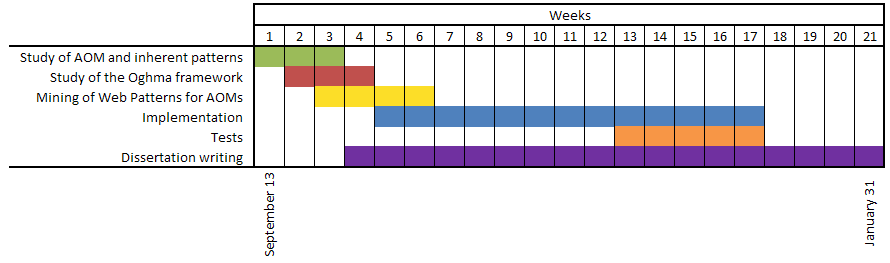
\includegraphics[width=\textwidth]{work_plan}
  \caption{Work plan for the duration of the thesis}
  \label{fig:work_plan}
\end{figure}

\section{Oghma and Design Patterns}\label{sec:oghma_and_design_patterns}

As the Oghma framework will act as the engine behind the interfaces to be developed, it is crucial that a solid knowledge of its API is acquired. Not only that, a careful study of the Oghma interface generation techniques must be performed in order to comprehend how the backend links itself with the user interfaces.

\section{Mining of Web Patterns for AOMs}\label{sec:mining_of_web_patterns}

This stage will be concerned with studying what the most effective GUI patterns are for applications of this type. A user should not perceive he or she is actually modifying the elementary structure of the system. As such, the user interface should be as intuitive as possible, with as less interference with the normal user workflow as possible. An initial study will be performed regarding current customization systems present in a multitude of websites --- what real-life paradigms and manipulation mechanisms are most commonly used, and try to transpose them to an AOM interface.

\section{Tasks}\label{sec:tasks}

This section will present a detailed list of all the major tasks planned for the next five months, as depicted in Table \ref{table:tasks}:

\begin{table}[H]
  \centering
  \begin{tabular}{c|c|c}
    \textbf{Task Description} & \textbf{Starting Date} & \textbf{Duration}\\
    \hline
    \hline
    Oghma API study                                   & September 20, 2010  & 2 weeks\\\hline
    Oghma interface generation                        & October 4, 2010     & 2 weeks\\\hline
    Studying current paradigms of web customization   & October 4, 2010     & 1.5 weeks\\\hline
    Adapting current paradigms to AOM interfaces      & October 13, 2010    & 2 weeks\\\hline
    QUALQUER COISA PARA COMPLETAR ISTO                & DATA                & DATA\\\hline
  \end{tabular}
  \vspace{3mm}
  \caption{Detailed tasks descriptions and durations}
  \label{table:tasks}
\end{table}

